%==================================================================%
% Author : Pando Muñoz, Manuel                                     %
%          Sánchez Barreiro, Pablo                                 %
% Version: 1.0, 30/03/2011                                         %
%                                                                  %
% Memoria del Proyecto Fin de Carrera                              %
% Archivo raíz para el capítulo de la arquitectura del sistema     %
%==================================================================%


\chapterheader{Arquitectura y diseño}{Definición Arquitectónica y Diseño Software}
\label{chap:arquitectura}

En el presente capítulo se presentan, mediante diagramas UML, la arquitectura física del sistema, los módulos, las comunicaciones entre ellos existentes en el sistema, y el funcionamiento del mismo.

\todo{finalizar breve introducción}

\chaptertoc

\section{Arquitectura física del Sistema}
\label{sec:arquitectura:arqFisica}

En esta sección se describe la arquitectura física del sistema mediante un diagrama de despliegue.
\begin{figure}
    \centering
    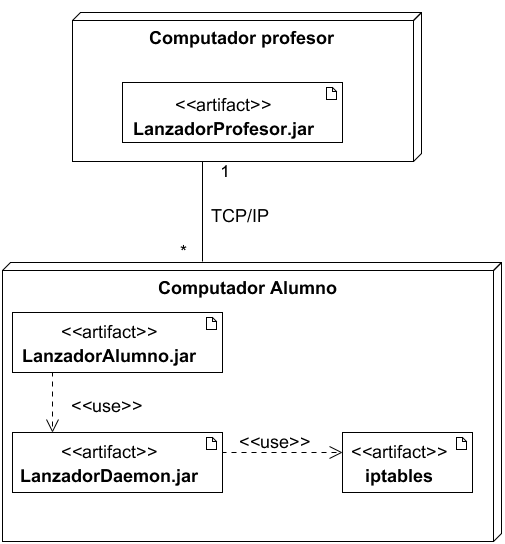
\includegraphics[width=\linewidth]{arquitectura/despliegueSistema2}
    \caption{Diagrama de despliegue del sistema}
    \label{fig:arquitectura:despliegueSistema}
\end{figure}
\newline


\lq\lq LanzadorProfesor.jar\rq\rq contiene lo necesario para mostrar la interfaz de usuario en la aplicación del profesor, así como la lógica de manejo de eventos y comunicación con las aplicaciones de los alumnos.

\lq\lq LanzadorAlumno.jar\rq\rq contiene las funciones para mostrar la interfaz de usuario de la aplicación del alumno, el manejo de eventos producidos por su uso y la lógica de comunicación con la aplicación del profesor y el demonio local.

\lq\lq LanzadorDaemon.jar\rq\rq contiene la lógica de comunicación con la aplicación del alumno y lo necesario para interactuar con iptables.

\lq\lq iptables\rq\rq es parte del núcleo del sistema Linux sobre el que se ejecutará la aplicación.

Cómo se puede puede observar, sólo se permite la existencia de una aplicación en el computador del profesor, a la que se conectan mediante TCP/IP un número indefinido de aplicaciones alumno, lógico, ya que en cada prueba suele haber varios los alumnos realizándola y uno el número de profesores.
\newline

A su vez, la aplicación del alumno interactúa con un único demonio del sistema.


\section{Diseño Software}
\label{sec:arquitectura:diseno}

En está sección se muestra un diagrama de actividad que resume las posibles interacciones que tanto el alumno como el profesor realizan con sus respectivas aplicaciones durante el trascurso normal de una prueba y un diagrama de estados para clarificar la aplicación del alumno.
\newline


\begin{figure}
    \centering
    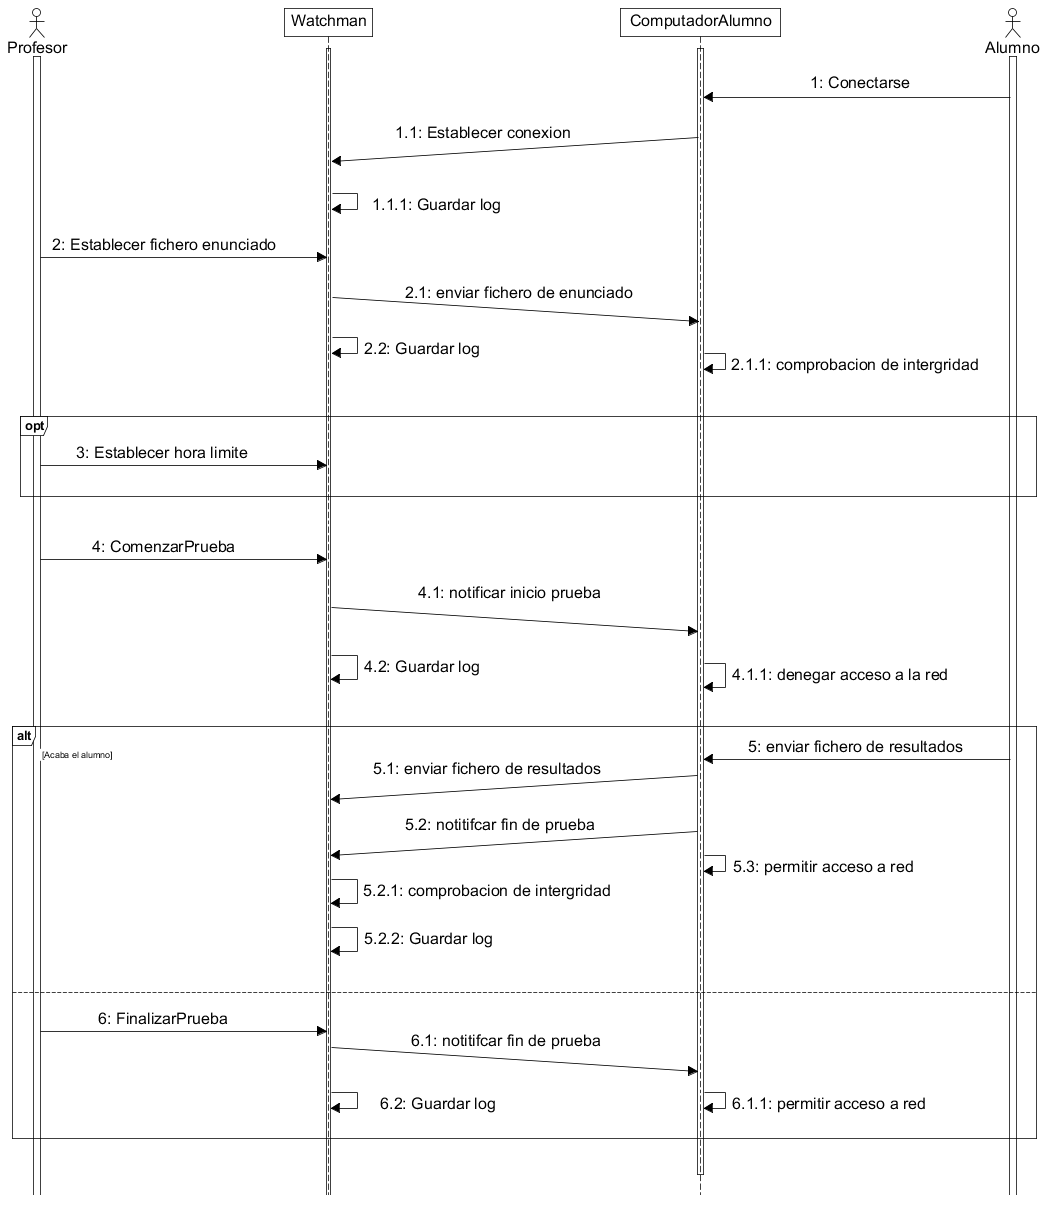
\includegraphics[width=\linewidth]{arquitectura/actividadSistema3}
    \caption{Diagrama de actividad del sistema}
    \label{fig:arquitectura:actividadSistema}
\end{figure}


Vemos en la figura \ref{fig:arquitectura:actividadSistema} que se siguen los pasos descritos en la sección \ref{sec:planificacion:descFuncional}



\begin{figure}
    \centering
    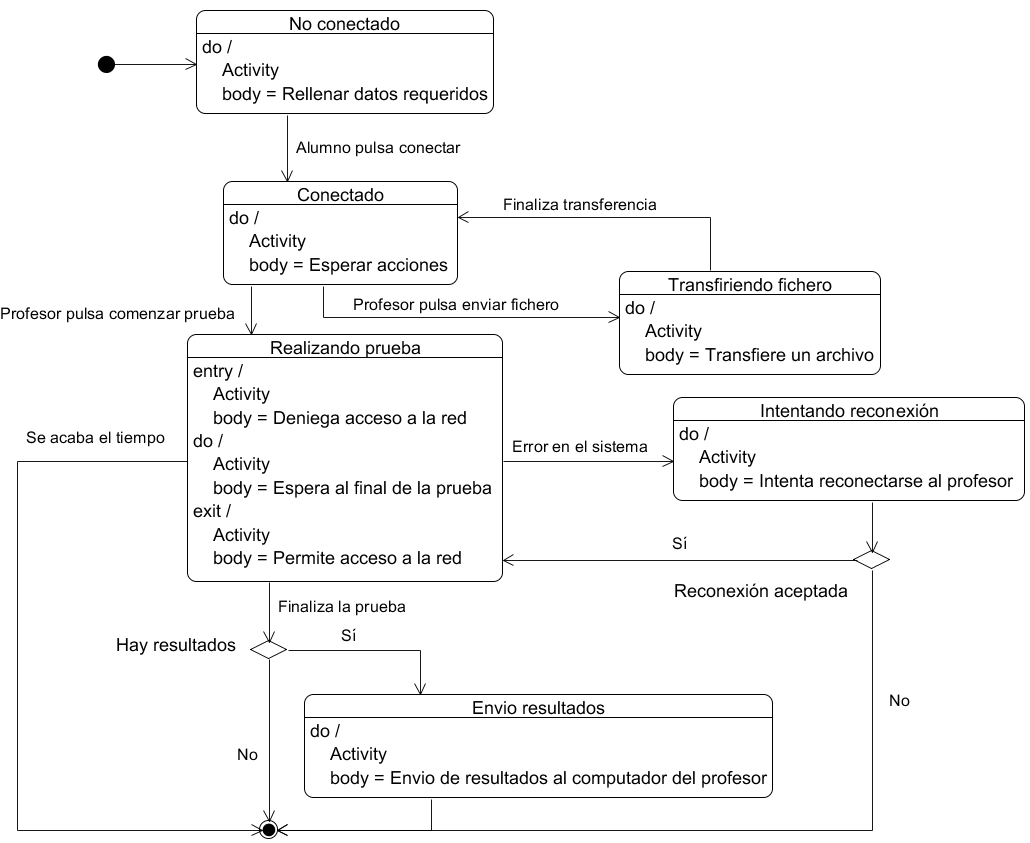
\includegraphics[width=\linewidth]{arquitectura/estadosAlumno2}
    \caption{Diagrama de estados de la aplicación del alumno}
    \label{fig:arquitectura:estadosAlumno}
\end{figure}


%Los estados se corresponden directamente con el estado en que se encuentra la prueba.

En la figura \ref{fig:arquitectura:estadosAlumno} se describe mediante un diagrama de estados el protocolo a implementar en la aplicación del alumno que ha de garantizar la principal funcionalidad de la aplicación, denegar el acceso a la red en los computadores de los alumnos que están realizando la prueba, mientras la prueba esté en marcha, sin necesidad de apagar el router o switch del laboratorio. 
\newline

El acto desactivar la red se consigue por medio de iptables, sección \ref{sec:introduction:iptables}, cambiando la política de los paquetes salientes una vez que empieza la prueba y hasta que acaba.
\newline

Por defecto iptables permite todo el tráfico que entre y salga del equipo, modificando las reglas para que deseche cualquier paquete destinado a cualquier equipo, conseguimos que no se pueda realizar ninguna petición a ningún nodo de la red, y, por tanto, tampoco recibiremos el contenido de la posible respuesta, el equipo del alumno queda aislado del resto.
\newline

A la hora de volver a permitir el acceso a la red, basta con modificar la política para el tratamiento de los paquetes salientes y restaurarla al estado anterior. Un alumno corriente no puede realizar esta operación ya que son necesarios privilegios de administrador para ello, por tanto, una vez que la aplicación desactiva la red, un alumno no puede interactuar con iptables para activarla de nuevo.
\newline


Vemos en la imagen que el único modo de finalizar la prueba es partiendo de una prueba ya iniciada, lógicamente, es decir, desde el estado \lq\lq Realizando prueba\rq\rq. Nada más entrar en este estado se desactiva el acceso a la red, por tanto, si se pretende finalizar la prueba, se ha tenido que realizar la misma sin acceso a la red.
\newline

Para entrar en el estado \lq\lq Realizando prueba\rq\rq, se pueden seguir dos caminos. El normal implica conectar la aplicación del alumno con la aplicación del profesor, cosa que únicamente se puede hacer antes de que de comienzo la prueba, por tanto, tampoco se puede realizar la prueba con acceso a la red y al finalizarla, conectarse y enviar los resultados, la aplicación no aceptaría la conexión.
\newline

El otro camino involucra a una funcionalidad que tiene el sistema que consiste en permitir reconexiones de alumnos que estuviesen realizando la prueba y por el motivo que sea, un error en el sistema, por ejemplo, hayan tenido que reiniciar el computador, cuándo la aplicación del alumno vuelva a ejecutarse, al inicio de la sesión automáticamente, se reconectará con la aplicación del profesor. En la imagen se observa que sólo se puede reconectar si previamente se estaba realizando la prueba y al reconectar volveríamos automáticamente a ese estado, en el que la red se desactiva al entrar, es decir, que aunque se reinicie el computador del alumno durante el transcurso de la prueba no se conseguiría acceso a la red.
\newline


%Otro punto importante es el de la recogida de resultados automática, se ha de garantizar que el archivo no se ha corrompido a lo largo de la transferencia, para ello se realizan, tanto en el equipo que envía el fichero como en el que lo recibe, firmas MD5 al mismo para comprobar que no ha habido errores en la transferencia.


